\begin{posterblock}{white}{smugold}{smunavy}{smucream}{M. Methods: Design-to-Test Logic Chain}
\compacttable
\renewcommand{\arraystretch}{1.12}
\begin{tabular}{@{}>{\bfseries}p{0.25\linewidth}p{0.18\linewidth}p{0.44\linewidth}@{}}
\toprule
Starting point & Value & Why it matters \\
\midrule
Selected profile & $e_r=1.0$, $e_w=5.0$, $\lambda=0.651$ & best-performing geometry from the previous design screen \\
Sheet and material & 316L, $t=1.2$ mm & thin metallic primary-barrier candidate \\
Patent basis & CN118237450A & coupled downward pressing and lateral squeezing for equal-section cross corrugation \\
\bottomrule
\end{tabular}

\vspace{0.6ex}
\begin{center}
\resizebox{0.92\linewidth}{!}{%
\begin{tikzpicture}[
  wflow/.style={rounded corners=4pt,minimum width=5.25cm,minimum height=1.28cm,align=center,font=\bfseries\small},
  arr/.style={-{Latex[length=3mm]},line width=0.9pt,draw=black!52}
]
\node[wflow,draw=smublue,fill=smublue!10] (s1) at (0,0) {1. Profile\\{\scriptsize previous best}};
\node[wflow,draw=smugold,fill=smugold!12] (s2) at (6.4,0) {2. Patent process\\{\scriptsize die + side extrusion}};
\node[wflow,draw=smugold,fill=smugold!12] (s3) at (12.8,0) {3. Samples\\{\scriptsize form + cut}};
\node[wflow,draw=smucyan,fill=smucyan!11] (s4) at (12.8,-2.05) {4. DIC first\\{\scriptsize strain release}};
\node[wflow,draw=smured,fill=smured!10] (s5) at (6.4,-2.05) {5. AE next\\{\scriptsize damage evolution}};
\node[wflow,draw=smunavy,fill=smunavy!10] (s6) at (0,-2.05) {6. Assembly\\{\scriptsize LN$_2$ cycles}};
\draw[arr] (s1.east) -- (s2.west);
\draw[arr] (s2.east) -- (s3.west);
\draw[arr] (s3.south) -- (s4.north);
\draw[arr] (s4.west) -- (s5.east);
\draw[arr] (s5.west) -- (s6.east);
\end{tikzpicture}}
\end{center}

\begin{center}
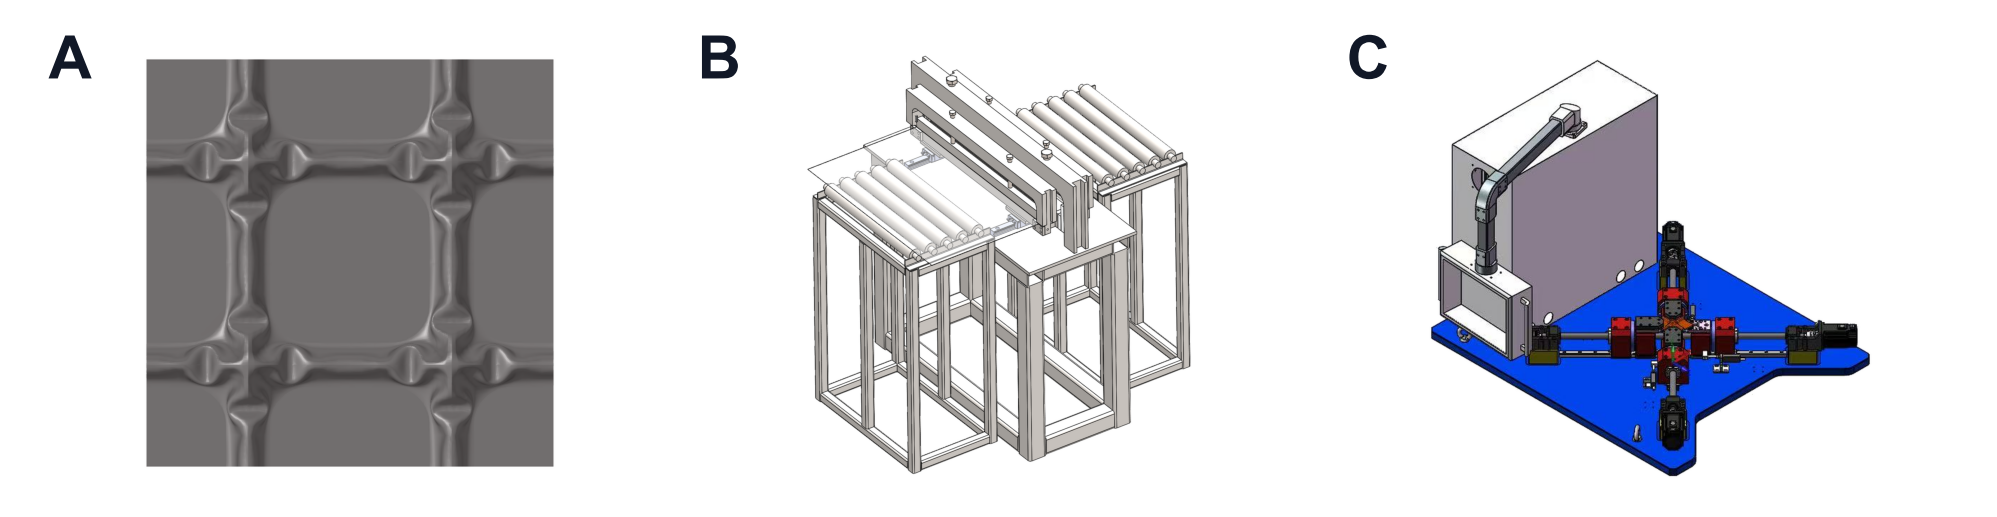
\includegraphics[width=\linewidth]{assets/fig02_uploaded_model_process_overview.png}
\end{center}
\smallnote{Selected profile $\rightarrow$ patented processing machine $\rightarrow$ four-axis specimen platform. The process figure is used as design and preparation context, not as a dimensional CAD claim.}

\vspace{0.7ex}
\begin{center}
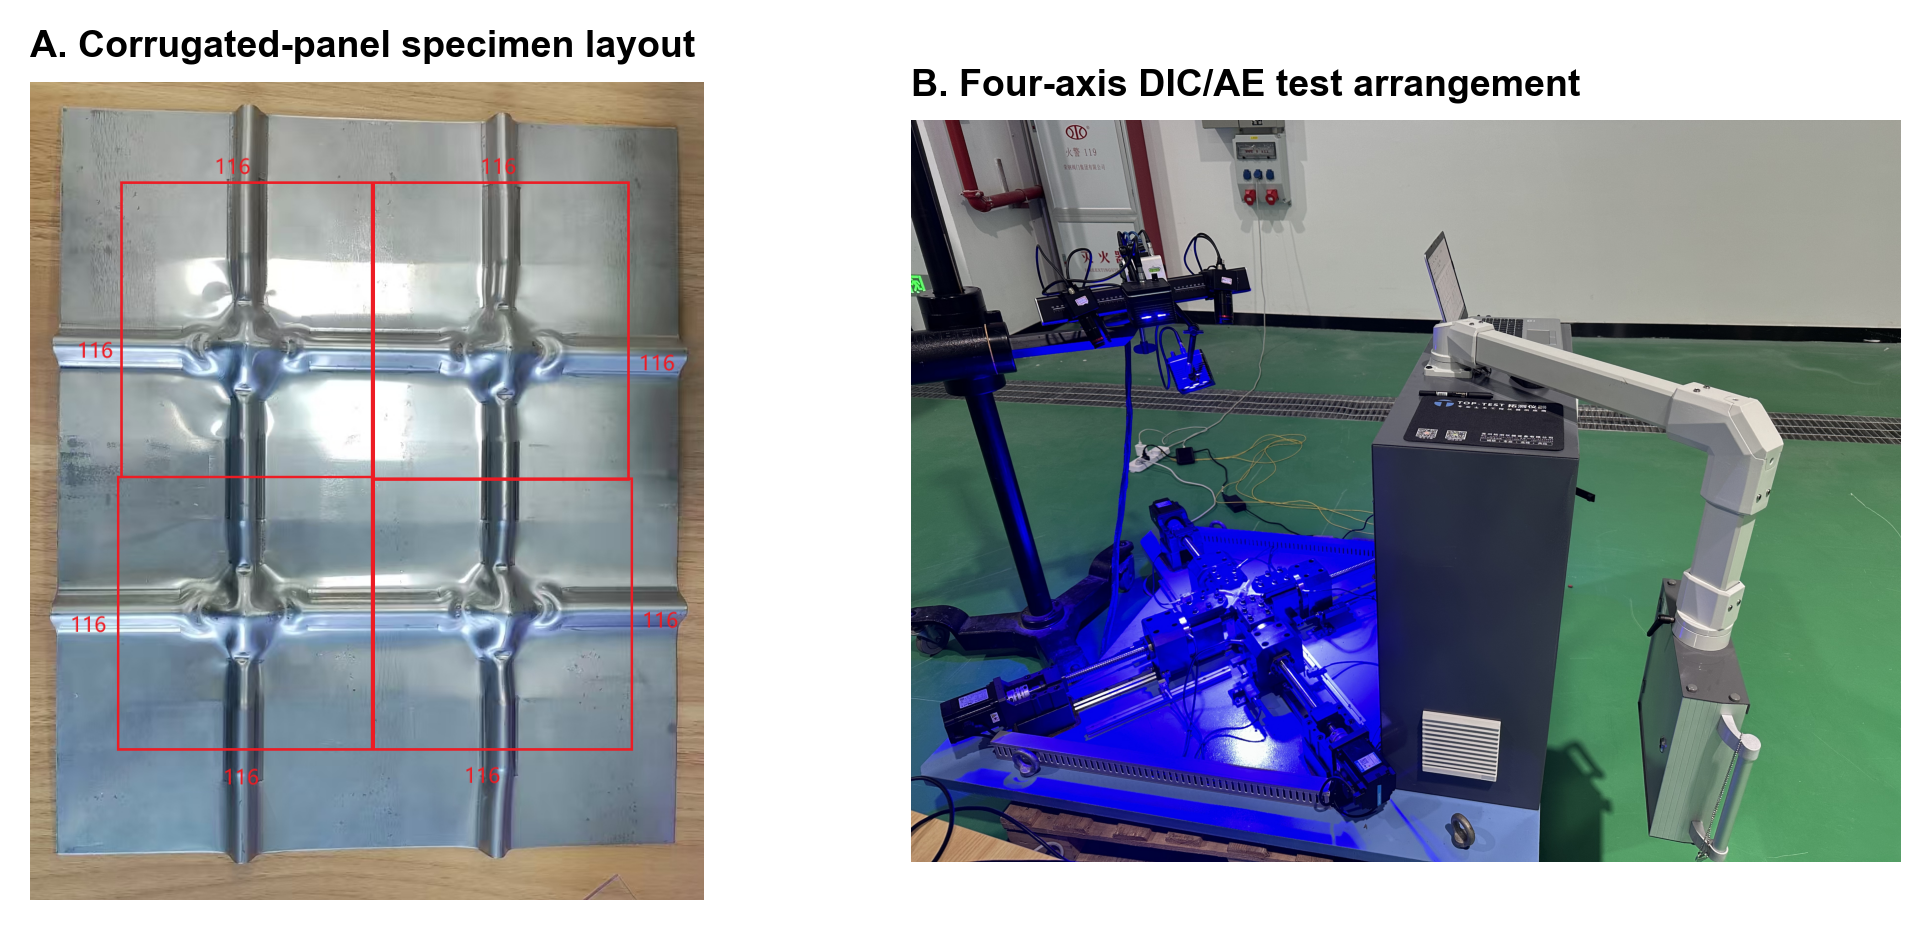
\includegraphics[width=\linewidth,height=18.0cm,keepaspectratio]{assets/fig02_experimental_setup_context.png}
\end{center}
\smallnote{Specimen extraction, DIC field of view, and mechanical setup connect the formed profile to the DIC/AE tests.}

\vspace{0.5ex}
\compacttable
\renewcommand{\arraystretch}{1.12}
\begin{tabular}{@{}>{\bfseries}p{0.20\linewidth}p{0.33\linewidth}p{0.35\linewidth}@{}}
\toprule
Experiment & Direct question & Measured output \\
\midrule
DIC/PLC & How does corrugation release imposed strain? & synchronized strain span, geometry-fixed ROI hierarchy \\
AE & When does cyclic activity concentrate? & relabeled cycle windows and damage-evolution screen \\
LN$_2$ assembly & Does pressure-retention testing verify assembly integrity after thermal cycling? & pressure-hold and helium leak checks across five LN$_2$ cycles \\
\bottomrule
\end{tabular}

\[
\bar{u}_k=\frac{1}{4}\sum_{a=1}^{4}u_{a,k},
\qquad
S_i=\frac{dP_{95}(|\varepsilon_x|)_i}{d\bar{u}},
\qquad
\Psi_i=A_iq_i^2
\]
\smallnote{The evidence chain is deliberately ordered: profile and processing first, DIC mechanism second, AE damage-evolution screening third, and pressure-retention testing for assembly integrity last.}
\end{posterblock}
